\documentclass[tikz,border=5pt]{standalone}
\usepackage{tikz}
\usetikzlibrary{positioning,arrows.meta,shapes.geometric,calc}

\begin{document}
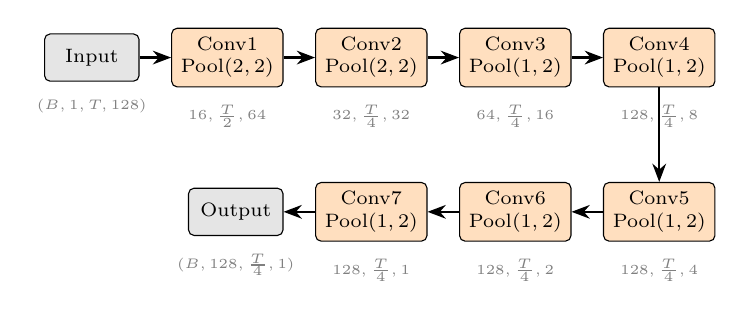
\begin{tikzpicture}[
    node distance=0.4cm,
    block/.style={rectangle, draw, fill=orange!25, minimum width=1.2cm, minimum height=0.7cm, align=center, rounded corners=2pt, font=\scriptsize},
    io/.style={rectangle, draw, fill=gray!20, minimum width=1.2cm, minimum height=0.6cm, align=center, rounded corners=2pt, font=\scriptsize},
    arrow/.style={-{Stealth}, thick},
    dimlab/.style={font=\tiny, text=gray}
]

% === Upper row: Input -> Conv1-4 ===
\node[io] (input) {Input};
\node[dimlab, below=0.1cm of input] {$(B, 1, T, 128)$};

\node[block, right=of input] (conv1) {Conv1\\Pool$(2,2)$};
\node[dimlab, below=0.1cm of conv1] {$16,\frac{T}{2},64$};

\node[block, right=of conv1] (conv2) {Conv2\\Pool$(2,2)$};
\node[dimlab, below=0.1cm of conv2] {$32,\frac{T}{4},32$};

\node[block, right=of conv2] (conv3) {Conv3\\Pool$(1,2)$};
\node[dimlab, below=0.1cm of conv3] {$64,\frac{T}{4},16$};

\node[block, right=of conv3] (conv4) {Conv4\\Pool$(1,2)$};
\node[dimlab, below=0.1cm of conv4] {$128,\frac{T}{4},8$};

% === Lower row: Conv5-7 -> Output ===
\node[block, below=1.2cm of conv4] (conv5) {Conv5\\Pool$(1,2)$};
\node[dimlab, below=0.1cm of conv5] {$128,\frac{T}{4},4$};

\node[block, left=of conv5] (conv6) {Conv6\\Pool$(1,2)$};
\node[dimlab, below=0.1cm of conv6] {$128,\frac{T}{4},2$};

\node[block, left=of conv6] (conv7) {Conv7\\Pool$(1,2)$};
\node[dimlab, below=0.1cm of conv7] {$128,\frac{T}{4},1$};

\node[io, left=of conv7] (output) {Output};
\node[dimlab, below=0.1cm of output] {$(B, 128, \frac{T}{4}, 1)$};

% Arrows - upper row
\foreach \i/\j in {input/conv1, conv1/conv2, conv2/conv3, conv3/conv4} {
    \draw[arrow] (\i) -- (\j);
}
% Arrow from conv4 to conv5 (going down)
\draw[arrow] (conv4) -- (conv5);
% Arrows - lower row
\foreach \i/\j in {conv5/conv6, conv6/conv7, conv7/output} {
    \draw[arrow] (\i) -- (\j);
}

\end{tikzpicture}
\end{document}
